% ---------------------------------------------------------------
% Task 2: Unsupervised Domain Adaptation
% Requires in the preamble:
%   \usepackage{graphicx,booktabs,amsmath,amssymb,siunitx}
%   \graphicspath{{figures/}}
% ---------------------------------------------------------------

\section{Unsupervised Domain Adaptation}
\label{sec:task2}

\subsection{Problem setting}

A classifier trained on photographs does not stay accurate when the test images
are pencil sketches. The object categories are unchanged, but the low-level
statistics that the network learned to rely on, colour, texture and shading, are
largely absent from a line drawing. Unsupervised domain adaptation (UDA) studies
what can be done about this when labelled examples exist only for the original
domains and the new domain arrives without any labels at all. The practical
appeal is obvious: unlabelled images are cheap, labelled ones are not.

This section asks whether four training objectives of increasing structure
actually close that gap on a standard benchmark. We begin with ordinary
supervised training, which sees only the labelled domains and establishes how far
conventional empirical risk minimisation transfers on its own. Three adaptation
objectives follow. DAN adds a statistical penalty that pulls the two feature
distributions together. DANN trains a separate network to tell the domains apart,
then punishes the backbone for making that easy. CDAN conditions that same
adversarial signal on the classifier's own predictions. The ordering
matters, because each method is allowed to use more information about class
structure than the one before it, and the experiment is designed to isolate what
that extra information buys.

Two terms recur throughout. \emph{Marginal alignment} matches the overall feature
distributions $P(F(X))$ of the two domains without reference to class labels.
\emph{Class-conditional alignment} also uses predicted class structure, on
the argument that matching distributions without regard to class can align a dog
in one domain to a horse in another. A third term, \emph{domain separability},
is defined in Section~\ref{sec:t2-diagnostic}; it measures how much domain
information survives in the learned features.

\subsection{Methodology}

\subsubsection{Data and evaluation protocol}

All experiments use PACS, a benchmark of 9{,}991 images spanning seven object
classes (dog, elephant, giraffe, guitar, horse, house, person) drawn from four
visual domains: Photo, Art Painting, Cartoon and Sketch. We treat Sketch as the
target domain and the remaining three as labelled sources. Sketch is the hardest
of the four to reach from the others, since it discards colour and texture
entirely, which makes it a demanding test rather than a flattering one.

Within each source domain we draw a stratified 80/20 train/validation split under
seed 6304, so every class keeps its proportion in both halves. The three
validation splits (1{,}213 images in total) are the only labelled data used for
model selection. All 3{,}929 Sketch images form the unlabelled adaptation set:
the adaptation objectives see these images during training but never their
labels. Target labels are read exactly once, after every model, setting and
checkpoint has been fixed, and only to compute the final numbers reported here.
This is a transductive protocol, and no target-label signal reaches any training
or selection decision.

\subsubsection{Backbone and optimisation}

Every method fine-tunes the same network end to end: an ImageNet-pretrained
ResNet-18 whose 1000-way classifier is replaced by a seven-way linear head on the
512-dimensional pooled feature. Images are resized to $256 \times 256$, then
augmented with a random $224 \times 224$ crop and a horizontal flip during
training; evaluation uses the $224 \times 224$ centre crop. Inputs are normalised
with the statistics of the pretrained weights.

One departure from default fine-tuning deserves explanation. Batch-normalisation
running means and variances are frozen at their pretrained ImageNet values for
every method, while the scale and shift parameters $\gamma$ and $\beta$ remain
trainable. If the running statistics were allowed to update, they would be
estimated from batches containing both source and target images, so the
normalisation itself would start adapting to the target distribution. That is a
second, implicit alignment mechanism, and leaving it active would make it
impossible to attribute any improvement to the alignment loss under study.
Freezing the statistics keeps the comparison honest. We verified the constraint
directly: the batch-normalisation buffers in all four saved checkpoints are
bitwise identical.

Training uses AdamW at learning rate $10^{-4}$ and weight decay $10^{-4}$ for at
most 30 epochs, stopping after five consecutive epochs without an improvement in
mean source-validation macro-F1. The checkpoint restored at the end of training
is the one that maximised that same quantity. Each update draws eight images from
each source domain and 24 target images, so source and target contribute equally
to any alignment term. Initialisation, sampling, augmentation policy, optimiser
and budget are held fixed across methods, and only the alignment objective
changes.

\subsubsection{Alignment objectives}

The \textbf{Source-only} baseline minimises cross-entropy over the three labelled
domains and never sees a target image. It measures how far ordinary supervised
learning transfers without any adaptation, and it doubles as the reference point
against which every later number is read.

\textbf{DAN} adds a statistical discrepancy penalty between the source and target
features immediately before the classifier head:
\begin{equation}
\mathcal{L}_{\mathrm{DAN}}
  = \mathcal{L}_{\mathrm{cls}}
  + \lambda_{\mathrm{MMD}}
    \bigl\lVert \mathbb{E}_s[\phi(F(x_s))] - \mathbb{E}_t[\phi(F(x_t))] \bigr\rVert^2_{\mathcal{H}} .
\end{equation}
The squared maximum mean discrepancy is evaluated through a sum of three RBF
kernels,
$k(u,v) = \sum_{m \in \{0.5,\,1,\,2\}} \exp\!\left(-\lVert u-v \rVert^2 / (m\,\tilde{d})\right)$,
where $\tilde{d}$ is the median pairwise squared distance in the current combined
batch. Using the kernel trick avoids ever constructing the feature map $\phi$.
The bandwidth is recomputed each batch and detached from the graph, so no
gradient flows through the median. We use $\lambda_{\mathrm{MMD}} = 1$ for the
main comparison. This objective knows nothing about which target image belongs to
which class; it only asks that the two clouds of features overlap.

\textbf{DANN} replaces that explicit discrepancy with a learned one. A
discriminator (256 hidden units, ReLU, dropout 0.5, two outputs) is attached to
the same 512-dimensional feature and trained to separate pooled source examples
from target examples. A gradient-reversal layer sits between the backbone and the
discriminator: it is the identity on the forward pass and multiplies the gradient
by $-\alpha$ on the backward pass, so the discriminator improves while the
backbone is pushed to defeat it. The reversal strength follows the standard
schedule
\begin{equation}
\alpha(p) = \frac{2}{1 + \exp(-10p)} - 1, \qquad p \in [0,1],
\end{equation}
with $p$ the fraction of the training budget consumed. Early on the backbone is
left alone to learn the class task; the adversarial pressure arrives once the
representation is already useful. Only source examples contribute to the
classification loss, while both domains contribute to the domain loss, which
carries unit weight.

\textbf{CDAN} keeps that machinery and changes only what the discriminator sees.
Instead of the feature $f = F(x)$ alone, it receives the flattened outer product
of the feature with the classifier's softmax vector $p = C(f)$,
\begin{equation}
g(x) = \mathrm{vec}(f \otimes p) \in \mathbb{R}^{3584},
\end{equation}
so a source and a target image can only be judged similar when they agree on both
appearance and predicted class. Hidden width, activation, dropout, reversal
schedule and loss weight are identical to DANN, and neither $f$ nor $p$ is
detached. The DANN/CDAN contrast therefore isolates conditioning and nothing else.

\subsubsection{Domain separability diagnostic}
\label{sec:t2-diagnostic}

Accuracy alone cannot say whether an alignment loss did what it claimed to do, so
we measure the alignment directly. After every checkpoint is fixed, each backbone
is frozen and used to extract features from equal numbers of source-validation
and target images (1{,}213 each). Those features are split 70/30 under seed 6304
and a balanced logistic regression with $C=1$ is trained to predict which domain
a feature came from. Its held-out accuracy is the \emph{domain separability}
score. A value near 0.5 means the two domains are indistinguishable in feature
space; a value near 1.0 means a linear probe recovers the domain almost perfectly.

The score deliberately measures only one thing. It says how much domain
information survives, not whether class information survived with it, and
Section~\ref{sec:t2-discussion} shows why that distinction decides the
interpretation of the whole experiment.

\subsection{Results}

\subsubsection{The unadapted gap}

Table~\ref{tab:t2-main} gives the full comparison. Source-only training reaches
93.2\% mean accuracy across the three source validation splits and 61.2\% on
Sketch, a drop of 32.0 points. Macro-F1 falls further, from 92.9 to 56.7, and
that asymmetry is the first useful signal: if the gap were a uniform loss of
quality, accuracy and macro-F1 would fall together. Failure is concentrated in
particular classes.

\begin{table}[t]
\centering
\caption{Task 2 comparison. Source columns are validation accuracy and macro-F1
within each labelled domain. Sketch is the unlabelled target, evaluated once
after all checkpoints were fixed. $\Delta$ is the change in target accuracy
relative to Source-only. Separability is the held-out accuracy of a linear domain
probe, where 0.5 is chance. All values except separability are percentages.}
\label{tab:t2-main}
\small
\setlength{\tabcolsep}{4pt}
\begin{tabular}{lcccccccccccc}
\toprule
& \multicolumn{2}{c}{Photo} & \multicolumn{2}{c}{Art Paint.} & \multicolumn{2}{c}{Cartoon}
& \multicolumn{2}{c}{Source mean} & \multicolumn{2}{c}{Sketch} & &  \\
\cmidrule(lr){2-3}\cmidrule(lr){4-5}\cmidrule(lr){6-7}\cmidrule(lr){8-9}\cmidrule(lr){10-11}
Method & Acc & F1 & Acc & F1 & Acc & F1 & Acc & F1 & Acc & F1 & $\Delta$ & Sep. \\
\midrule
Source-only & 95.8 & 94.8 & 90.5 & 90.1 & 93.4 & 93.9 & 93.2 & 92.9 & 61.2 & 56.7 & --- & 0.997 \\
DAN         & 95.5 & 94.3 & 94.1 & 93.9 & 94.2 & 94.4 & 94.6 & 94.2 & \textbf{62.7} & \textbf{57.3} & $+1.5$ & 0.853 \\
DANN        & 46.8 & 25.3 & 33.2 & 18.2 & 38.0 & 31.8 & 39.3 & 25.1 & 16.5 & 9.2 & $-44.7$ & 0.966 \\
CDAN        & 52.3 & 41.2 & 32.0 & 24.1 & 42.9 & 39.2 & 42.4 & 34.8 & 15.7 & 9.8 & $-45.6$ & 0.995 \\
\bottomrule
\end{tabular}
\end{table}

Table~\ref{tab:t2-perclass} and Figure~\ref{fig:t2-perclass} identify where.
The Source-only model recognises elephants almost perfectly on Sketch (99.6\%
recall) and persons almost never (2.5\%, four images out of 160). That pairing is
not a coincidence. Elephant absorbs 1{,}959 of the 3{,}929 target predictions
against a true support of 740, giving it a precision of 0.376. The confusions
that feed it are systematic: 453 of 772 dogs, 334 of 816 horses, 214 of 753
giraffes and 133 of 160 persons are all labelled elephant. A grey, texture-free
outline on white paper resembles the model's internal notion of an elephant more
than it resembles anything else, so one class quietly swallows the target domain.
Reporting accuracy alone would hide this behind a single high-recall class, which
is precisely why the protocol tracks macro-F1.

\begin{table}[t]
\centering
\caption{Per-class behaviour on the 3{,}929 Sketch images. Recall is the fraction
of each class recovered; precision is the fraction of predictions for that class
that are correct. Precision is shown for the two methods that trained
successfully, since it exposes the absorbing-class failures that recall alone
conceals.}
\label{tab:t2-perclass}
\small
\begin{tabular}{lrcccccc}
\toprule
& & \multicolumn{2}{c}{Source-only} & \multicolumn{2}{c}{DAN} & DANN & CDAN \\
\cmidrule(lr){3-4}\cmidrule(lr){5-6}\cmidrule(lr){7-7}\cmidrule(lr){8-8}
Class & Support & Rec. & Prec. & Rec. & Prec. & Rec. & Rec. \\
\midrule
Dog      & 772 & 0.328 & 0.695 & 0.462 & 0.723 & 0.677 & 0.165 \\
Elephant & 740 & 0.996 & 0.376 & 0.734 & 0.784 & 0.000 & 0.008 \\
Giraffe  & 753 & 0.595 & 0.858 & 0.724 & 0.830 & 0.000 & 0.000 \\
Guitar   & 608 & 0.885 & 0.985 & 0.715 & 1.000 & 0.028 & 0.671 \\
Horse    & 816 & 0.467 & 0.784 & 0.551 & 0.939 & 0.000 & 0.000 \\
House    &  80 & 0.562 & 0.957 & 1.000 & 0.140 & 0.363 & 0.900 \\
Person   & 160 & 0.025 & 0.800 & 0.331 & 0.088 & 0.494 & 0.013 \\
\bottomrule
\end{tabular}
\end{table}

\begin{figure}[t]
\centering
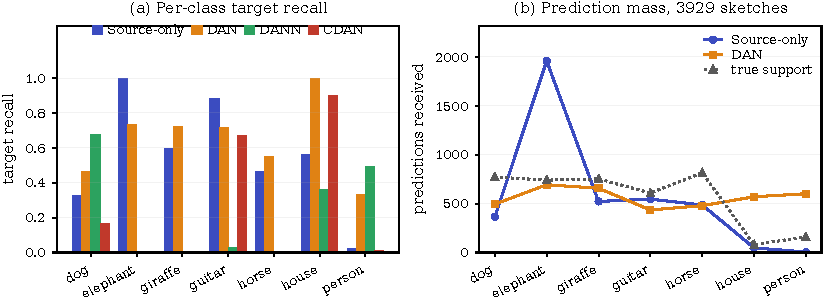
\includegraphics[width=\textwidth]{per_class.pdf}
\caption{(a) Per-class recall on the Sketch target. (b) How the 3{,}929 target
predictions are distributed across classes, against the true class supports.
Source-only piles predictions onto elephant; DAN removes that pile and creates a
smaller one on house and person.}
\label{fig:t2-perclass}
\end{figure}

\subsubsection{Statistical alignment}

DAN improves target accuracy from 61.2\% to 62.7\%. Taken alone that increase of
1.5 points looks marginal, and the per-class view shows it understates what
changed. DAN dismantles the elephant sink, lifting its precision from 0.376 to
0.784, and recovers classes the baseline had abandoned: person rises from 0.025
to 0.331 recall, dog from 0.328 to 0.462 and giraffe from 0.595 to 0.724. Source
performance also improves slightly (93.2\% to 94.6\%), so the gain does not come
from trading source accuracy away. Domain separability falls from 0.997 to 0.853,
confirming that the MMD penalty made the two feature distributions genuinely
harder to tell apart.

The improvement is smaller than those per-class numbers suggest because DAN
introduces a new failure of the same kind. House, with a true support of 80,
receives 570 predictions at a precision of 0.140, and person receives 601 at a
precision of 0.088. The absorbing class moved rather than disappeared.
Figure~\ref{fig:t2-perclass}(b) shows this directly: Source-only concentrates
mass on elephant, DAN spreads mass far more evenly but overshoots on the two
smallest classes. This is the behaviour marginal alignment is expected to produce.
The objective asks only that the two feature clouds overlap, and it is satisfied
by mapping target images onto whichever source region is nearest, whether or not
that region carries the right label.

\subsubsection{Adversarial alignment}

Both adversarial runs failed to train. DANN reaches 39.3\% mean accuracy and
CDAN 42.4\% on the source domains they are directly supervised on, against 93.2\%
for the baseline. A model that cannot fit its own labelled training domains has
not traded target performance for invariance; it has failed to optimise. We
report these runs as an optimisation failure rather than as negative transfer,
and the distinction matters for how the numbers should be read.

Figure~\ref{fig:t2-training} shows the mechanism. Both runs collapse within the
first few epochs onto a characteristic equilibrium. The classification loss
settles at roughly 1.91, against $\ln 7 = 1.946$ for a uniform guess over seven
classes. The domain loss settles at roughly 0.694, against $\ln 2 = 0.693$ for a
discriminator that cannot separate 24 source from 24 target images. Reaching chance on the domain loss looks like successful
confusion until it is read alongside the classification loss. The discriminator
is at chance because the features have collapsed and there is nothing left in
them to discriminate. DANN then diverges numerically, with both losses exceeding
$10^{8}$ by epoch 20.

Three observations locate the cause in the objective rather than in the
implementation. First, a control run of DANN with the maximum reversal strength
set to zero, which trains the discriminator but sends no reversed gradient to the
backbone, trains normally and reaches 0.929 mean source-validation macro-F1. The
reversed gradient is therefore the only difference between a healthy run and a
collapsed one. Second, DAN shares every other component of the pipeline and
trains without difficulty. Third, DAN itself collapses in the same way when its
alignment weight is raised far enough (Section~\ref{sec:t2-strength}), which
shows the failure is driven by the magnitude of alignment pressure rather than by
anything specific to adversarial training.

The objective admits this behaviour by construction. Cross-entropy is unbounded
above, so instructing the backbone to maximise the domain loss sets it an
optimisation problem with no finite solution: it can always do better by driving
the discriminator further into confident error. Adam compounds the problem,
because it rescales gradients to a roughly fixed step size and so grants the
adversarial direction a full-sized step even while $\alpha$ is still small.
Backbone and discriminator share a single learning rate, so the backbone can
outrun the opponent it is supposed to be fighting. The frozen
batch-normalisation statistics remove the one mechanism that would otherwise
rescale drifting activations. The original formulation of DANN avoids this with
stochastic gradient descent under an annealed learning-rate schedule, which the
fixed optimiser used here rules out.

One consequence is worth stating plainly, because it determines whether the
reported numbers are meaningful. Checkpoint selection on source-validation
macro-F1 retained epoch 15 for DANN and epoch 12 for CDAN, both of which precede
the numerical divergence. The saved weights sit 12.2\% and 12.8\% away from the
Source-only checkpoint in relative $L_2$ distance, with the movement concentrated
in the middle of the network (0.104 and 0.141 for layer2 and layer3 in DANN,
against 0.059 and 0.103 for DAN). The rows in Table~\ref{tab:t2-main} therefore
describe a collapsed but numerically well-behaved model, not the diverged state.

\begin{figure}[t]
\centering
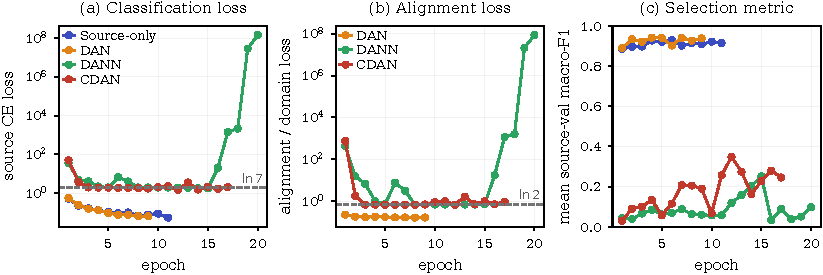
\includegraphics[width=\textwidth]{training_dynamics.pdf}
\caption{Training dynamics. (a) Source classification loss, log scale, with
$\ln 7$ marking a uniform guess over seven classes. (b) Alignment loss, log
scale: weighted MMD for DAN and domain cross-entropy for DANN and CDAN, with
$\ln 2$ marking a discriminator at chance. (c) Mean source-validation macro-F1,
the quantity used for early stopping and checkpoint selection. DANN and CDAN
settle onto the $\ln 7$ / $\ln 2$ pair within a few epochs, and DANN then diverges.}
\label{fig:t2-training}
\end{figure}

\subsubsection{Alignment strength}
\label{sec:t2-strength}

To test how the amount of alignment pressure changes the outcome, we swept
$\lambda_{\mathrm{MMD}} \in \{0.1, 1, 10\}$ for DAN with every other setting
fixed. Table~\ref{tab:t2-lambda} and Figure~\ref{fig:t2-strength}(a) report the
sweep.

\begin{table}[t]
\centering
\caption{DAN alignment-strength sweep. Every other setting is held fixed.
Accuracies are percentages; separability is the linear domain probe, chance
$=0.5$.}
\label{tab:t2-lambda}
\small
\begin{tabular}{lcccc}
\toprule
$\lambda_{\mathrm{MMD}}$ & Mean source acc. & Target acc. & Separability & Epochs run \\
\midrule
0.1 & 94.0 & \textbf{67.6} & 0.982 & 8 \\
1   & \textbf{94.6} & 62.7 & 0.853 & 9 \\
10  & 21.7 & 4.1  & 0.514 & 6 \\
\bottomrule
\end{tabular}
\end{table}

The three settings behave very differently. At $\lambda = 0.1$ the penalty is
light, separability stays high at 0.982, and target accuracy reaches its best
value of 67.6\%, an improvement of 6.4 points over the baseline. At $\lambda = 1$
alignment bites harder, separability drops to 0.853, and target accuracy falls
back to 62.7\%. At $\lambda = 10$ the representation collapses outright: the MMD
term reaches exactly zero by epoch four, which can only happen when every feature
in a batch is identical, separability falls to 0.514, and target accuracy drops to
4.1\%. That last figure is exactly $160/3929$, the support of the person class,
because the model assigns every one of the 3{,}929 target images to a single
label.

Because the sweep must be resolved without target labels, the selection question
has a definite answer. Ranking the three settings by mean source-validation
accuracy picks $\lambda = 1$ at 94.6\%, ahead of $\lambda = 0.1$ at 94.0\% and far
ahead of the collapsed $\lambda = 10$ at 21.7\%. Source validation therefore
rejects the catastrophic setting correctly but forfeits 4.9 points of target
accuracy by preferring $\lambda = 1$ to $\lambda = 0.1$. The signal available
without target labels is enough to avoid disaster and not enough to find the
optimum.

\begin{figure}[t]
\centering
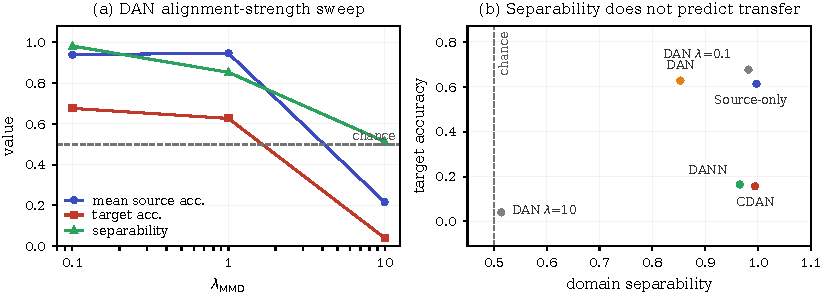
\includegraphics[width=\textwidth]{strength_study.pdf}
\caption{(a) Effect of $\lambda_{\mathrm{MMD}}$ on source accuracy, target
accuracy and domain separability. (b) Target accuracy against domain
separability for all six trained configurations. The relationship is
non-monotone in both directions, so separability on its own does not predict
transfer.}
\label{fig:t2-strength}
\end{figure}

\subsection{Discussion}
\label{sec:t2-discussion}

\paragraph{The gap is a class-structure problem, not a uniform loss of quality.}
Moving from the labelled domains to Sketch costs 32.0 points of accuracy and 36.2
points of macro-F1. The larger fall in macro-F1 is the diagnostic. The model does
not degrade evenly; it collapses onto a small number of classes, with elephant
receiving 1{,}959 of 3{,}929 predictions at a precision of 0.376 while person
receives five. The entropy of the predicted label distribution makes the same
point compactly: 1.430 nats for Source-only against a maximum of
$\ln 7 = 1.946$. Any aggregate improvement on this benchmark has to be checked
against the per-class breakdown, because a method can raise accuracy simply by
choosing a better class to over-predict.

\paragraph{Lower domain separability does not imply better transfer.}
Figure~\ref{fig:t2-strength}(b) plots the two quantities against each other for
all six trained configurations, and the relationship fails in both directions.
DAN at $\lambda = 10$ achieves a separability of 0.514, within a point and a half
of chance, and is the worst model we trained at 4.1\% target accuracy; it reached indistinguishable
domains by destroying the features that distinguished anything at all. DANN and
CDAN fail the converse way, with adversarial training in place and separability
still at 0.966 and 0.995, because collapsed features remain domain-separable even
when they are useless for classification. The only configuration that both lowered
separability and improved transfer is DAN at $\lambda = 1$, and even there the best
target accuracy in the whole study came from $\lambda = 0.1$, whose separability
was the second highest of the six. A separability score is interpretable only
alongside the classification loss and source accuracy, never on its own.

\paragraph{Conditioning changed stability rather than semantics.}
CDAN outperformed DANN on every measure of training health. Its best
source-validation macro-F1 was 0.348 against 0.251, its mean source accuracy 42.4\%
against 39.3\%, it escaped the collapse plateau where DANN stayed pinned, and its
domain loss never exceeded $7.6 \times 10^{2}$ where DANN reached
$8.6 \times 10^{7}$. Since the two differ only in the conditioning, that gap is
attributable to conditioning. It is not, however, evidence that conditioning
preserved semantic structure. The two models produce prediction distributions of
almost identical entropy, 1.054 nats for CDAN against 1.025 for DANN, both far
below Source-only's 1.430 and DAN's 1.933, and both collapse onto two or three
absorbing classes. Whatever conditioning bought, it was not class structure.

There is a mechanism for the stability difference that has nothing to do with
semantics, and it follows from the geometry of the outer product. Since
$\lVert f \otimes p \rVert_F = \lVert f \rVert_2 \lVert p \rVert_2$ and
$\lVert p \rVert_2$ ranges from $1/\sqrt{7}$ for a uniform prediction to $1$ for a
confident one, the conditional discriminator receives a systematically smaller
input than the marginal one. Accounting for the $1/\sqrt{\text{fan-in}}$
initialisation, the ratio of CDAN's initial pre-activation scale to DANN's is
$\lVert p \rVert_2 \sqrt{512/3584} = \lVert p \rVert_2 / \sqrt{7}$, which equals
exactly $1/7$ when predictions are uniform. The attenuation is strongest precisely
when the classifier has collapsed, so CDAN damps its own adversarial pressure at
the moment DANN's runs away. That is a useful property, but it is a consequence of
input scaling, not of class-conditional matching.

The degenerate case closes the argument. When the classifier collapses to a
near-uniform $p$, which is what the loss curves show, $\mathrm{vec}(f \otimes p)$
becomes seven redundant copies of $f/7$, and the discriminator's first linear
layer reduces exactly to a $512 \to 256$ map on $f$. CDAN becomes DANN with a
rescaled input. Conditioning is computed from the classifier's own output, so it
carries information only when the classifier already works, and it offers no
protection during the collapse it would need to prevent. Our runs give no support
to the claim that conditioning preserves semantic structure, and they show why the
mechanism cannot be expected to help in this regime.

\paragraph{The only method that helped used the weakest form of alignment.}
DAN at $\lambda = 0.1$ produced the best target accuracy in the study, 67.6\%,
using a non-adversarial penalty applied gently enough to leave separability at
0.982. The two objectives with access to more structure, an adversarial
discriminator and a class-conditional one, both destroyed the representation under
the prescribed optimiser. On this benchmark, under this budget, the returns to
sophistication were negative.

\subsection{Limitations}

Each configuration was trained once under a single seed, so the DANN and CDAN
stability difference is one observation rather than a measured effect. The
attenuation argument describes initialisation and the collapsed regime; the
discriminator can learn to compensate for the input scale over training, and we
did not measure how quickly it does. Most importantly, because neither adversarial
run converged, we cannot say how conditional alignment compares to marginal
alignment when both train successfully. The comparison reported here is between
two failure modes, and the question of whether conditioning preserves semantic
structure in a converged model remains open under this protocol.
